\section{Boundary attachments and vanishing boundary effects}
\label{sec:boundary}

The construction below joins two nearby boundary points by a nonnegative
path and completes it through a suitable part of the genuine exterior
to surround a small boundary neighborhood.  We call the resulting
separator a boundary arch.  Its failure probability will decay
exponentially in the number of available scales.  Searches from the
small-neighborhood side will then remove the exceptional windows in the
pinning brackets.  Searches from the opposite side will control an
absolute height average near the boundary while leaving distant height
observations measurable outside the arch.

The first task is to attach a nonnegative path to a prescribed boundary
arc.  A bulk circuit alone does not give that attachment.  We construct
a lower comparison law whose mean near the arc is close to $-1/2$;
a level-path exploration then forces a boundary-attached zero path with
positive probability.  Every real separating site retains its actual
height throughout these comparisons.

\subsection{The boundary convention and a synthetic lower trace}

Write $V_\delta$ for the set of face centers on which the finite height
problem is defined, including its prescribed boundary sites, and write
$S_{0,\delta}$ for the connected boundary walk of
Lemma~\ref{lem:boundary-walk}.  We use its image as a graph; occurrences
of one vertex in the traversal are not different height variables.
If a further site circuit is exposed, the \emph{usable trace} of a
retained component consists of its real fixed neighboring sites.  The
values at those sites remain part of the conditioning.

For a height $H$ and a level $t$, put
\begin{equation}
 \widehat{\mathcal O}_t(H)
 = (\delta\T\setminus V_\delta)
   \,\cup\,\{v\in V_\delta:H(v)\ge t\}.
 \label{boundary:artificial-exterior}
\end{equation}
Thus only sites outside the \emph{original} height problem are declared
open artificially.  A real vertex which is removed during a search is
still a real vertex, with its observed height.  For the reversed
convention replace $H\ge t$ by $H\le t$.

Here and below every geometric length is positive and fixed before the
mesh limit.  In tangent and inward normal coordinates at
$p\in\partial D$, let $Q_a(p)=p+[-a,a]^2$.  There is a radius, uniform in
$p$, on which the limiting boundary is a graph with any prescribed
small slope tolerance.  Parametric convergence has two further uses.
First, all portions of $S_{0,\delta}$ in a fixed local box lie in a
vanishing neighborhood of the corresponding limiting arc.  Second,
two visits belonging to a smaller boundary patch can be joined along
the walk in a slightly larger patch.  Both assertions have fixed
positive slack; they do not assert that the discrete boundary is a
graph.  To connect such a patch to the genuine exterior, take a lattice
path from a point on its exterior side towards an interior point and
stop at its first boundary site.  Join that site to the desired
boundary endpoint along the walk in the larger patch.  To justify this
local connection, choose a slightly larger limiting arc containing the
smaller patch.  The inverse of the limiting Jordan
parametrization is uniformly continuous.  Hence, for fine mesh, all
visits to the smaller patch occur in the corresponding traversal
interval, up to its fixed endpoint slack.  The intervening walk stays
in the larger patch by uniform parametric convergence.  This applies
to repeated visits as well as distinct vertices.

For the lower comparison, use $W$ as the first color.  Its plus sign
can represent the pair $\{-1,0\}$ and its minus sign the pair
$\{-3,-2\}$.  We place the first pair near a clean boundary arc and
the second pair elsewhere.  An open-plus cut near the clean arc will
then permit reflection of the inner height about $-1/2$.  The following
construction fixes these actual integer pairs with only finitely many
component labels, even when the discrete boundary walk has many repeated
visits.  This bounded label count is what keeps the later circuit
estimates uniform.

\begin{lemma}[Synthetic trace]\label{boundary:synthetic-trace}
Fix finitely many high and low boundary arcs, separated by transition
neighborhoods of positive length, with both types present.  The high
cores and all their transition neighborhoods lie where the usable actual
trace is at least zero; the remaining usable trace is at least $-2$.
One may also add real separator pieces, each connected piece meeting
its low part and staying a positive distance from the high cores and
their transition neighborhoods.  There may be arbitrarily many such
pieces, for example when two site circuits enter and leave the domain
many times.  For all sufficiently small meshes there is a synthetic
height $K$, obtained from a free
ambient spin law by first-color pins and at most $M$ second-color
labels, such that its connected prescribed skeleton $S$ has trace
\begin{equation}
 K|_{S^+}\in\{-1,0\},\qquad
 K|_{S^-}\in\{-3,-2\}.
 \label{boundary:synthetic-pairs}
\end{equation}
Here $S=S^+\cup S^-$, the high part contains the high cores and stays
inside their prescribed larger arcs, and $M$ depends only on the
number of these arcs.  It does not depend on the separator pieces, the
length of the discrete walk or the number of its repeated vertices.
Given its full trace, $K$ has the usual height Gibbs laws in the
bounded faces of $S$, and these laws are below the actual laws in
height order.  Before imposing the second-color labels, an event
measurable in the first color and its statuses whose failure
probability is $\varepsilon$ has failure probability at most
$2^M\varepsilon$ after they are imposed.
\end{lemma}

\begin{proof}
Choose shortened cores of the prescribed arcs, leaving disjoint
transition neighborhoods between consecutive cores.  The image of an
appropriate consecutive portion of the boundary traversal gives a
connected graph for each core.  Compact limiting cores of opposite
types are separated, so their images neither intersect nor have an
edge between them at sufficiently small mesh.  Any portion not yet
assigned is in one of the transition neighborhoods.  Repeated visits
inside a core belong to that same connected core image.  Any repeated
visit that could affect assignment outside the cores is localized to
a transition neighborhood: otherwise two traversal parameters a fixed
positive distance apart would converge to the same point of the Jordan
curve.  Uniform continuity of its inverse parametrization excludes
this possibility.

Grow the connected core sets in the finite walk graph.  For example,
give each unassigned vertex to a nearest core in graph distance,
breaking ties in a fixed order, and use a shortest path to that core
as its parent.  Each resulting part is connected.  Each component of
the still unassigned graph had a neighboring core, since the entire
walk graph is connected; hence the procedure assigns every vertex.
The growth stays in the transition neighborhoods until it meets an
already assigned core.  In particular it never changes a prescribed
core or its type.  Merge neighboring parts of the same type.  Added
separator pieces are assigned low and joined to the low parts they
meet.  Their clearance from the high patch makes this consistent.
Every added piece attaches to an existing low part, so it creates no
new part; it may merge existing low parts.  In particular no cost is
charged for the number of real components of an added circuit.

Pin $W=+$ or $W=-$ on the resulting parts.  Their adjacency graph is
connected.  On each edge of a spanning tree joining opposite-sign
parts, choose one corresponding skeleton edge and prescribe $B=-$
there.  Its two endpoints already have opposite $W$ signs, so
coherence forces their $B$ signs to agree.  There are at most $M$
such labels.  Anchor the lift by $K(o)=-1$ at a plus endpoint of one
of these edges.  Along a connected constant-$W$ part the lifted pair
is unchanged; a labeled transition changes $-1$ to $-2$.  Propagation
along the spanning tree therefore gives
\eqref{boundary:synthetic-pairs}.  Extra contacts between parts create
no further choice of lift: the ambient lift is single valued.  The
configuration $B\equiv-$ shows that all the imposed conditions are
simultaneously feasible.  The separate flat comparison below fixes
both spins and does not use this construction.

Conditional on $W$ and its statuses, the $B$ components have fair
independent labels.  Requiring at most $M$ of them to have label minus
has conditional probability at least $2^{-M}$, even if several
requests refer to the same component.  This proves the last
assertion.  The height Gibbs property follows on conditioning on the
whole trace and integrating out the statuses.  On each high part
the synthetic trace is at most zero, and on each low part it is at
most $-2$.  Lemma~\ref{lem:height-order} gives the claimed comparison
on every retained component.
\end{proof}

For later stopping arguments it is useful to state the elementary
site-circuit fact explicitly.

\begin{lemma}[Extremal site circuits]\label{boundary:extremal}
In a specified finite annular strip, consider the simple open site
circuits surrounding a fixed connected inner box.  If one exists,
there is an innermost and an outermost such circuit, ordered by their
geometric Jordan interiors.  Selection of the innermost circuit
requires only its trace and observations on its inner side in the
strip; selection of the outermost requires only its trace and
observations on its outer side.  Artificial openness as in
\eqref{boundary:artificial-exterior} does not change these assertions.

Consequently, inner circuits selected from the inside and outer
circuits selected from the outside in disjoint strips leave the
pairwise disjoint unexamined middle components with their height Gibbs laws, independent
given the revealed data and their real traces.
\end{lemma}

\begin{proof}
Two eligible cycles have inner and outer envelopes made of edges in
their union.  To see this, if they share at least two vertices, their
union is two-vertex-connected.  Indeed, after deleting any vertex,
each cycle is connected and at least one common vertex remains.
The face of this union containing the inner box and its unbounded
face have simple cycle boundaries.  They give the required
envelopes.  The inner box is connected and disjoint from the cycles,
so it lies in a single face.  If the cycles have no common vertex or
only one, the requirement that both surround the box makes them
nested.  In every case the envelopes stay in the original strip
and surround its inner box.  Finitely many repeated envelopes give
the least and greatest Jordan interiors.  Geometric interiors, not
just sets of enclosed lattice vertices, determine this order.

For a proposed innermost circuit $\gamma$, the assertion that it is
selected is equivalent to its being open and to the nonexistence of
an eligible open circuit with strictly smaller interior contained
in its interior.  A nonnested competitor would give such a circuit
by the inner-envelope operation.  The equivalent assertion reads
only the sites on or inside $\gamma$ in the strip.  The outer case
is identical with the order reversed.  Deterministic tie conventions
for a traversal of the selected cycle do not reveal additional
sites.  An unsuccessful strip can be read in its entirety.

All these selection events are consequently measurable in the
discarded regions and the separating traces.  The nearest-neighbor
height density factors over the remaining components, proving the
Gibbs and independence claims.  Only the goodness test of a genuinely
exterior site is deterministic.  Every selected real site retains
its actual observed height in this factorization.
\end{proof}

\subsection{A local attachment}

We isolate the probabilistic and topological step which joins a bulk
path to the actual boundary.  Its constants are uniform over the
separator traces allowed in the statement.

\begin{lemma}[Attachment to a clean arc]\label{lem:boundary-attachment}
There are constants $\lambda>0$ and $a_0>0$, depending only on $x$,
with the following property.  Fix $b>0$ and put $s=\lambda b$.
Suppose a retained height problem has a connected bounding skeleton
consisting of $S_{0,\delta}$ and separator pieces, all with usable
trace at least $-2$.  A clean local patch of the base skeleton has
trace at least zero.  Use tangential and inward-normal coordinates
$(t,y)$ at this patch, and call $y$ its depth.  Assume that all its
base-skeleton sites in the box $|t|\le 2b$, $|y|\le b$ lie in
$|y|<s/10$, the added separators miss the box, and the compact part
above that band is in the domain.  The high core and all transition
sites can be chosen within $|t|<b/3$, with a core covering $|t|\le b/8$.

At all sufficiently small meshes, uniformly in the retained trace,
the probability of an actual
path of heights at least zero from the clean base patch to depth
$s$, staying in $|t|<b$, is at least $a_0$.  Its boundary endpoint
can be joined, through real nonnegative boundary sites in a slightly
larger clean patch, to the artificially open exterior.
\end{lemma}

\begin{proof}
Choose $s/b$ small, to be fixed at the end of the proof.  Apply
Lemma~\ref{boundary:synthetic-trace} with one high patch as stated and
the rest of the skeleton low.  The separators are low and meet the
low base part, so the number $M$ of transition labels is bounded by
an absolute constant.  Work first with this synthetic height $K$ in
a large free ambient triangulation containing the local boxes.  Any
sufficiently large finite volume suffices: after conditioning on the
full skeleton trace, the interior height law is independent of that
ambient volume.  All estimates below are uniform in this choice.
Let $z$ be a lattice site at distance $O(\delta)$ from $(0,3s)$.

\paragraph{The successful cut and its reflection.}
Look for a good $W$-plus cut surrounding $z$ between an inner box of
radius $4s$ and an outer box of radius $b/16$.  Slight fixed changes
of these numerical radii accommodate lattice rounding.  The inner
box also contains a site $v$ of the high core.  The annular buffers
meet only favorable plus pins, and all transition labels lie outside
the outer box.  The stack estimate of
Lemma~\ref{lem:buffer-circuits}, followed by the bounded label cost,
gives an event $G$ with
\begin{equation}
 \Prob(G^c)\le \eta(s/b),\qquad
 \eta(u)\le C u^{\alpha},
 \label{boundary:cut-failure}
\end{equation}
for some $C,\alpha>0$.  The event and the choice of cut are measurable
in $W$ and its statuses.

Given these variables and the prescribed transition labels, every
$B$ component inside the good cut is free and no such component
crosses it.  Flip all their labels.  On the connected pinned high
part one has
\[
 K(v)-\tfrac12B(v)=-\tfrac12.
\]
Consequently this flip sends $K(v)$ to $-1-K(v)$.  All increments
inside the cut also change sign, since $W$ is unchanged and $B$ is
reversed.  It follows throughout its protected interior that
\begin{equation}
 K\longmapsto-1-K.
 \label{boundary:minus-half-reflection}
\end{equation}
This is a weight-preserving involution of the still fair component
labels.  In particular the conditional mean at $z$, on $G$, is
exactly $-1/2$.

\paragraph{Why failure has bounded conditional mean.}
Let $\mathcal A$ contain the full first color and its statuses and
the prescribed second-color labels.  Increments satisfy
\begin{equation}
 \dd(K-BW/2)=-B\,\dd W.
 \label{boundary:component-identity}
\end{equation}
For each $B$ component $C$, the portion of $\dd W$ carried by that
component has zero curl.  Every $W$-changing edge belongs to a closed
cell.  The two changing edges of any triangle share a vertex, so
their endpoints belong to the same $B$ component and their
contributions cancel.  Its potential $\phi_C$ has oscillation at most two:
on $C$ it equals $W$ up to a constant, and outside $C$ it is
constant until a path first hits $C$.  This is also the
component-potential calculation in Lemma~\ref{lem:collar-switch}.
Integrating \eqref{boundary:component-identity} from the labeled
anchor $o$, where $K(o)=-1$, gives an endpoint correction of absolute
value at most one and one term
$-B_C(\phi_C(z)-\phi_C(o))$ for each component.  Every unlabeled
component has conditional mean zero.  At most $M$ components are
labeled.  Therefore
\begin{equation}
 \big|\E[K(z)\mid\mathcal A]\big|\le 2+2M.
 \label{boundary:failure-mean}
\end{equation}
Since $G$ is $\mathcal A$-measurable, its failure contributes at most
$(2+2M)\Prob(G^c)$ to the \emph{mean}.  No pointwise height bound or
bound on $\E[|K(z)|\mid G^c]$ is being used.  Combining
\eqref{boundary:minus-half-reflection}--\eqref{boundary:failure-mean}
shows that
\begin{equation}
 \left|\E K(z)+\tfrac12\right|\le C_M\eta(s/b).
 \label{boundary:synthetic-mean}
\end{equation}

\paragraph{Boundary-entering level paths and a Gibbs ceiling.}
Condition on the synthetic height trace on $S$ and consider the
bounded face containing $z$.  Starting at every trace edge with
values $-1,0$, follow its dual level path at level $-1/2$, stopping
when it returns to the skeleton.  Reveal only the path and its two
adjacent site lips.  Continuation is unique: in a triangle containing
an edge with values $-1,0$, the third height is either $-1$ or $0$,
so exactly two of its edges cross this level.  Such a path cannot
branch or turn into an independent closed contour.  Stop a path also
at an earlier revealed segment if necessary, and exhaust all the
boundary-entering paths.  Each high lip is a connected chain of
zeros attached to a zero on the prescribed skeleton; each low lip
has height $-1$.

This is a stopped height exploration: the next query is determined
by the already revealed heights, so the unrevealed regions retain
their height Gibbs laws.  Give a remaining region the high or low
designation inherited from the side of the exposed paths and the
original trace.  This designation ignores every unexposed closed
contour.  It is consistent because a closed contour in a bounded
face cannot enclose part of the connected bounding skeleton, or
part of a path attached to that skeleton.  After all the entering
paths have been traced, a low region has usable boundary at most
$-1$, while a high region has usable boundary at most zero.  This
can alternatively define the designation by cutting the face along
the exposed paths and using their oriented lips.  If $z$ is itself
revealed, its lip gives the same bounds directly.

Height comparison with the constant ceilings $-1$ and $0$, whose
mean fields are respectively $-1$ and $0$, now gives
\begin{equation}
 \E K(z)\le -1+\Prob(z\hbox{ has the high designation}).
 \label{boundary:ceiling}
\end{equation}
An unseen closed contour can create a high island inside a
low-designated region.  Its entire Gibbs contribution is included
in this ceiling comparison; the high designation is not the event
$K(z)\ge0$.  Equations~\eqref{boundary:synthetic-mean} and
\eqref{boundary:ceiling} yield a high-designation probability at
least $1/2-C_M\eta(s/b)$.

\paragraph{The barriers force a real attachment.}
Figure~\ref{fig:boundary-attachment} depicts the following separation
argument.
At the two boundary projections $t=\pm2b/3$, request good $W$-minus
circuits in annuli with inner size $2s$ and outer size less than
$b/8$.  Choose the inner boxes to contain the whole cross-section
$-s/10\le y\le s$ at the corresponding projection.  Each annulus
meets only low skeleton pins; its circuit meets the low part and
therefore uses the anchored pair $\{-3,-2\}$.  Its adjacent site
path contains a surrounding site circuit of heights at most $-2$.
The same stack estimate and label cost bound the probability of
failure of either barrier by $2\eta_1(s/b)$, where
$\eta_1(u)\to0$.  These barrier events are intersected with the
high-designation event after deriving \eqref{boundary:ceiling}; they
were not extra observations in that Gibbs comparison.

Every exposed zero lip starts on the designated high patch: the
rest of $S$, including the added separators, has heights $-3,-2$.
Suppose no such lip reaches depth $s$ while $|t|<b$.  Before any
sideways exit its sites have depth less than $s+O(\delta)$, and
they cannot have depth less than $-s/10-O(\delta)$ locally because
they lie in the closure of the bounded face on the domain side of
the base boundary.  To pass the lateral projection $2b/3$, a lip
starting in $|t|<b/3$ would have to enter the inner box of the right
low circuit.  It starts outside that circuit, and planar site paths
cannot cross without sharing a vertex.  It would therefore meet a
site of height at most $-2$, impossible for a zero lip.  The left
barrier gives the other side.  This argument applies to the entire
lip, regardless of its number of visits to the shallow strip.
Thus all exposed boundary-entering contours are confined to
$|t|<2b/3+O(\delta)$ and $y<s+O(\delta)$.

There is now a path from $z$ at depth $3s$ along a horizontal
corridor to $t$ close to $b$, followed by a downward path towards
depth $-s$.  Choose nearest-neighbor lattice paths within
$O(\delta)$ of these segments and stop at the first real skeleton
site.  The horizontal corridor is inside the domain and above all
the confined exposed paths.  The descent lies beyond their
horizontal range.  Its proposed endpoint below the shallow band is
genuinely exterior, so the separation property of $S_{0,\delta}$
forces a first skeleton hit.  That hit is low, since its tangential
coordinate lies beyond the high patch and all transition zones.
No added separator enters this box.  Until the first hit the route
stays in the same face of $S$, even when that face has a boundary
walk with repeated vertices.  It crosses no exposed level path and
therefore connects $z$ to a low-designated boundary portion.  This
contradicts the high designation of $z$.  The low circuits themselves
need not be avoided by this route; they were not used to subdivide
the designation.

It follows that high designation and the two barriers force an
actual zero lip attached to the high patch to rise to depth $s$.
Choose $s/b=\lambda$ so small that
$C_M\eta(\lambda)+2\eta_1(\lambda)<1/4$.
The synthetic attachment then has probability at least $1/4$.
All slope tolerances and mesh errors are chosen only after this
positive ratio is fixed.

Finally the existence of a path of heights at least zero from this
patch to depth $s$ is an increasing height event.
Lemma~\ref{boundary:synthetic-trace} transfers its lower probability
to the actual retained law.  Its endpoint is a real clean boundary
site.  The local walk connection described above joins it to a
boundary site incident to the genuine exterior, using real clean
sites whose heights are all at least zero.  Only after this
connection do we use artificial openness outside $V_\delta$.
This proves the lemma, for instance with $a_0=1/4$.
\end{proof}

\begin{figure}[!htbp]
 \centering
 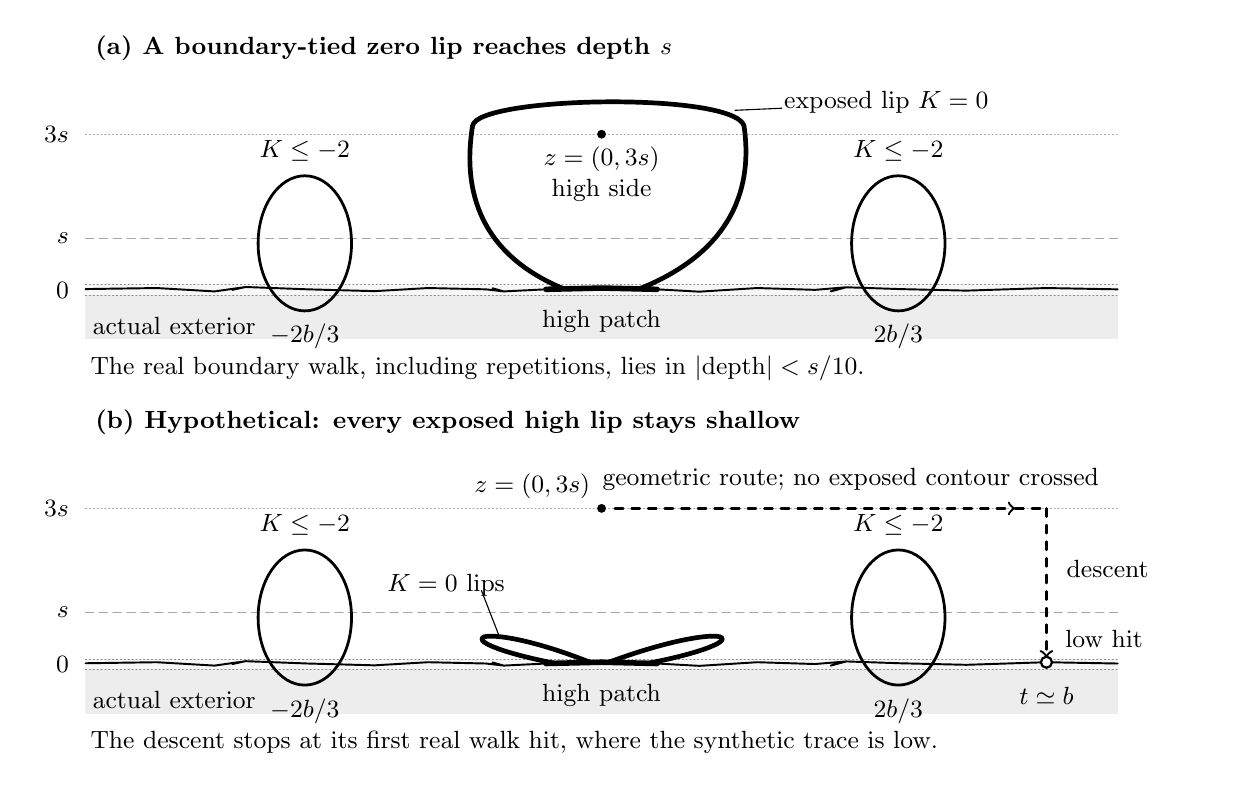
\begin{tikzpicture}[x=5.65cm,y=0.66cm,
  font=\fontsize{9}{11}\selectfont,line cap=round,line join=round]
\path[use as bounding box] (-1.29,-9.0) rectangle (1.36,5.05);
\foreach \panelshift in {0,-7.2} {
  \begin{scope}[shift={(0,\panelshift)}]
    \fill[black!7] (-1.16,-0.95) rectangle (1.16,-0.1);
    \fill[black!3] (-1.16,-0.1) rectangle (1.16,0.1);
    \draw[black!45,densely dotted] (-1.16,-0.1) -- (1.16,-0.1);
    \draw[black!45,densely dotted] (-1.16,0.1) -- (1.16,0.1);
    \draw[black!35,densely dashed] (-1.16,1) -- (1.16,1);
    \draw[black!35,densely dotted] (-1.16,3) -- (1.16,3);
    \node[anchor=east,fill=white,inner sep=1pt] at (-1.19,1) {$s$};
    \node[anchor=east,fill=white,inner sep=1pt] at (-1.19,3) {$3s$};
    \node[anchor=east,inner sep=1pt] at (-1.19,0) {$0$};
    \draw[line width=0.7pt]
      (-1.16,0.02) -- (-1.00,0.04) -- (-0.87,-0.025) -- (-0.80,0.06)
      -- (-0.83,0.005) -- (-0.80,0.06) -- (-0.66,0.015)
      -- (-0.51,-0.02) -- (-0.39,0.04) -- (-0.26,0.015)
      -- (-0.22,-0.025) -- (-0.245,0.035) -- (-0.22,-0.025)
      -- (-0.125,0.015) -- (0,0.04) -- (0.125,0.015)
      -- (0.22,-0.03) -- (0.35,0.04) -- (0.48,0.005)
      -- (0.55,0.055) -- (0.515,-0.025) -- (0.55,0.055)
      -- (0.67,0.02) -- (0.82,-0.01) -- (1,0.04) -- (1.16,0.015);
    \draw[line width=2pt] (-0.125,0.015) -- (0,0.04) -- (0.125,0.015);
    \draw[line width=1pt] (-0.667,0.9) ellipse [x radius=0.105,y radius=1.3];
    \draw[line width=1pt] (0.667,0.9) ellipse [x radius=0.105,y radius=1.3];
    \foreach \a in {-0.667,0.667} {
      \node[anchor=south,fill=white,inner sep=1pt] at (\a,2.42) {$K\le -2$};
    }
    \fill (0,3) circle [radius=1.6pt];
    \node[anchor=north] at (-0.667,-0.47) {$-2b/3$};
    \node[anchor=north] at (0.667,-0.47) {$2b/3$};
    \node[anchor=north,fill=black!7,inner sep=1pt] at (0,-0.32) {high patch};
    \node[anchor=west,inner sep=0pt] at (-1.145,-0.68) {actual exterior};
  \end{scope}
}
\node[anchor=west,font=\fontsize{9}{11}\selectfont\bfseries] at (-1.16,4.65)
  {(a) A boundary-tied zero lip reaches depth $s$};
\draw[line width=1.7pt]
  (-0.085,0.025) .. controls (-0.29,0.75) and (-0.31,2.1) .. (-0.29,3.16)
  .. controls (-0.28,3.73) and (0.29,3.82) .. (0.32,3.17)
  .. controls (0.34,2.03) and (0.30,0.76) .. (0.085,0.025);
\node[anchor=west,align=left,fill=white,inner sep=1.5pt] at (0.40,3.62)
  {exposed lip $K=0$};
\draw[thin] (0.405,3.5) -- (0.30,3.46);
\node[align=center,fill=white,inner sep=1.5pt] at (0,1.92) {high side};
\node[anchor=north,fill=white,inner sep=1.5pt] at (0,2.84) {$z=(0,3s)$};
\node[anchor=west,inner sep=0pt] at (-1.15,-1.50)
  {The real boundary walk, including repetitions, lies in $|\mathrm{depth}|<s/10$.};

\begin{scope}[shift={(0,-7.2)}]
  \node[anchor=west,font=\fontsize{9}{11}\selectfont\bfseries] at (-1.16,4.65)
    {(b) Hypothetical: every exposed high lip stays shallow};
  \node[anchor=south east,fill=white,inner sep=1.5pt] at (-0.015,3.1) {$z=(0,3s)$};
  \draw[line width=1.7pt]
    (-0.105,0.02) .. controls (-0.38,0.48) and (-0.28,0.91) .. (-0.025,0.035);
  \draw[line width=1.7pt]
    (0.015,0.035) .. controls (0.29,0.91) and (0.38,0.48) .. (0.105,0.02);
  \node[anchor=east,fill=white,inner sep=1pt] at (-0.21,1.53) {$K=0$ lips};
  \draw[thin] (-0.27,1.42) -- (-0.23,0.54);
  \draw[dashed,line width=0.85pt,->] (0.03,3) -- (0.93,3);
  \draw[dashed,line width=0.85pt,->] (1,3) -- (1,0.13);
  \draw[dashed,line width=0.85pt] (0.93,3) -- (1,3);
  \draw[fill=white,line width=0.8pt] (1,0.04) circle [radius=2pt];
  \node[anchor=south,fill=white,inner sep=2pt] at (0.56,3.23)
    {geometric route; no exposed contour crossed};
  \node[anchor=west,fill=white,inner sep=1.5pt] at (1.035,1.83) {descent};
  \node[anchor=west,inner sep=1pt] at (1.035,0.49) {low hit};
  \node[anchor=north,inner sep=1pt] at (1,-0.38) {$t\simeq b$};
  \node[anchor=west,inner sep=0pt] at (-1.15,-1.50)
    {The descent stops at its first real walk hit, where the synthetic trace is low.};
\end{scope}
\end{tikzpicture}

 \caption{The local attachment geometry, schematically and not to
 scale.  In the application to Proposition~\ref{prop:boundary-arch},
 the box lies near $(2\ell,0)$ in the untouched band
 $Q_{5\ell}\setminus Q_\ell$, away from the preliminary separators.
 Every local branch of the real boundary walk lies in the shallow
 tolerance band.  The high synthetic trace is in $[-1,0]$, the
 remaining trace in $[-3,-2]$.  Low ambient site circuits enclose the
 shallow cross-section near $t=\pm2b/3$.
 (a) An exposed zero lip attached to the high patch rises to depth
 $s$; ``high side'' is a contour-side designation, not a sign
 assertion for $K(z)$.
 (b) If every such lip stays shallow, the dashed geometric route
 reaches its first real low-trace site without crossing an exposed
 contour.  Unexposed closed contours remain integrated in the Gibbs
 law.  The exterior is joined only after a real attachment is obtained.}
 \label{fig:boundary-attachment}
\end{figure}
\FloatBarrier

\subsection{From attachments to many-scale boundary arches}

The local attachment will be joined to other attachments by paths in
the free bulk.  We establish that second ingredient before iterating
the construction across scales.

\begin{lemma}[Nonnegative paths through bulk tubes]
\label{boundary:bulk-tubes}
Consider a bounded face of a connected fixed skeleton, with its weighted
height law and usable trace at least $-2$.  Fix a finite network of
tubes in that face with positive widths and clearance from the skeleton.
Their lengths, widths and clearances are specified by fixed ratios.
For all sufficiently small meshes, the probability that every requested
tube is traversed in its prescribed direction by a site path of heights
at least zero is bounded below by a positive constant depending only
on $x$ and the network geometry.  The bound is uniform over the shape
of the skeleton outside these clearances and over its prescribed trace.
\end{lemma}

\begin{proof}
Compare from below with the flat trace $-2$ on the connected bounding
skeleton.  Realize this flat problem by
constant spin pins in the ambient graph.  In an allocated annulus
around a tube ball, ask for at least three nested good first-color
circuits with alternating signs, using disjoint buffers.  The
conditional buffer estimates give positive probability.  Constancy
of the other color on the connected skeleton is first imposed as
equality.  Its single component label is fair conditional on the
first color and its statuses.  Prescribing that label therefore leaves
the circuit-search probability unchanged.  Between successive
opposite-sign circuits there are enclosing first-color
walls, so there are at least two enclosing height loops in the
allocated annulus.  The loops lie wholly in the free bulk.

Let $E$ be the event that at least two enclosing height loops lie
wholly in the allocated annulus.  This event depends only on the
unoriented geometry and contains the alternating-color circuit event,
so its probability has the same positive lower bound.  Condition now
only on unoriented geometry in $E$.  Choose two consecutive enclosing
loops in the annulus by a deterministic rule, ordered from outer to
inner.  All loop jumps are
independent fair signs under the flat boundary, by
Lemma~\ref{lem:height-order}.  The height outside the first chosen
loop is $-2$ plus a symmetric sum of other signs, and hence is at
least $-2$ with probability at least $1/2$.  Independently, both
chosen jumps are positive with probability $1/4$.  With probability
at least $1/8$ their inner lip therefore supplies a surrounding
site circuit of height at least zero.  Each loop's two site lips
have constant heights: at every trivalent vertex on the loop the
third edge is unoccupied, joining the same-height sites along each
lip.  Loops not enclosing the
target ball cannot change this lip height.  A surrounding site
circuit can be extracted from its connected site walk.

The allocated annuli can be chosen so that successive surrounding
site circuits must intersect.  For example take equal inner radii
$a$, outer radii $2a$, and successive center distance $3a/2$.
The enclosed inner disks overlap, whereas either inner disk has a
portion beyond the other outer disk; disjoint surrounding circuits
could consequently be neither unnested nor nested.  After small
fixed changes to the radii for lattice rounding, planarity forces
an intersection.  Finite strings of these annuli give the desired
tube paths.  Each surrounding-height-circuit event is increasing,
so height association multiplies their lower bounds, first in the
flat problem and then in the actual problem by height comparison.
Only finitely many balls are needed for the fixed tube network.
\end{proof}

\begin{samepage}
\begin{proposition}[Boundary arch estimate]\label{prop:boundary-arch}
There are constants $L>100$, $c,C>0$ and a positive slope tolerance
such that the following holds.  Fix $p\in\partial D$ and a local
radius $R$ satisfying that tolerance.  Suppose the actual prescribed
trace on $S_{0,\delta}$ is at least $-1$ everywhere and at least zero
in $Q_R(p)\setminus Q_r(p)$.  Choose any $N$ positive scales
\[
 16r\le\ell_1,\qquad
 L\ell_j\le\ell_{j+1},\qquad
 \ell_N\le R/10.
\]
At all sufficiently small meshes,
\begin{equation}
 \Prob\!\left(
 \begin{array}{c}
 \text{a site circuit in }\widehat{\mathcal O}_0(H)
 \text{ surrounds }Q_r(p)\\[-2pt]
 \text{and is contained in }Q_R(p)\setminus Q_r(p)
 \end{array}\right)
 \ge 1-Ce^{-cN}.
 \label{boundary:arch-estimate}
\end{equation}
The constants are independent of $N,p$ and the prescribed trace;
the required mesh threshold may depend on the chosen positive
scales and the boundary approximation.  The same assertion holds
with all inequalities reversed when the original trace is at most
$1$ everywhere and at most zero in the clean annulus.  All usable
sites of the resulting arch have their real height at least zero,
or at most zero in the reversed assertion.
\end{proposition}
\end{samepage}

\begin{proof}
We give the increasing construction.  All choices of relative widths
below are fixed once and for all, depending at most on $x$.

\paragraph{Preliminary blocks at level $-1$.}
In block $j$ seek site circuits of level at least $-1$ in the two
strips
\[
 Q_{\ell_j}\setminus Q_{\ell_j/2},
 \qquad Q_{7\ell_j}\setminus Q_{5\ell_j},
\]
with artificial exterior allowed, each surrounding its inner box.
Use Lemma~\ref{boundary:synthetic-trace} with high intervals on the
two clean boundary subarcs running through \emph{all} these strips.
Place their transitions before the innermost buffers and beyond
the outermost ones, in the available clean annulus.  Low intervals
are used on the remaining skeleton.  There are only two high arcs,
so the number $M$ of transition labels is independent of $N$.

Before imposing those labels, the slightly narrower buffers in
each strip see only favorable first-color pins.  By
Lemma~\ref{lem:buffer-circuits} there is $a_1>0$ such that, given
the earlier complete first-color/status slot records, both good
plus circuits in the next block occur with conditional probability
at least $a_1$.  All such buffers are disjoint by the choice of $L$.
A good circuit meets a high boundary arc, since that arc traverses
the strip.  Its adjacent site path is consequently in the anchored
pair $\{-1,0\}$.  That path has winding number one around the inner
box; erasing unnecessary pieces gives a simple surrounding site
circuit at level at least $-1$.

If $I_j$ records the two-circuit success, the conditional estimate
implies, for $t>0$,
\[
 \E\exp\!\left(-t\sum_{j=1}^N I_j\right)
 \le(1-a_1+a_1e^{-t})^N.
\]
Choosing $t$ and then a sufficiently small $a_2>0$ gives
$\Prob(\sum I_j<a_2N)\le e^{-c_1N}$.
Conditioning on the bounded number of transition labels multiplies
this failure bound by at most $2^M$.  Thus with probability at least
$1-C_1e^{-c_1N}$ at least $a_2N$ blocks have both site circuits.
The event that at least this many blocks succeed is increasing in
the heights.  Height comparison transfers the entire count estimate
to the actual law, without conditioning successively on synthetic
events in that law.

In each actual successful block select an innermost circuit in the
inner strip and an outermost circuit in the outer strip.  Reveal
the unsuccessful strips and every nonretained region.  By
Lemma~\ref{boundary:extremal}, conditional on this record
$\mathcal R$, all retained middle components have independent height
Gibbs laws.  Their skeleton is the base skeleton together with the
real portions of the two selected circuits.  Each circuit surrounds
a boundary-centered box containing a point a fixed positive distance
outside $D$.  A site circuit lying wholly in the real domain would
have its geometric interior in the simply connected $D_\delta$,
so each selected circuit visits the genuine exterior.  Every maximal
real run along it therefore ends at a transition to the exterior;
its endpoint is a site of the original boundary face layer.  Thus
every connected real portion meets the base skeleton.  There can be
arbitrarily many such real portions.  In either local attachment
comparison they all meet low base sites, since the high patch lies
in the untouched middle band.  They can therefore be adjoined to
the existing low parts without creating new parts or new transition
labels, exactly as in Lemma~\ref{boundary:synthetic-trace}.
The resulting prescribed graph is connected.  Its usable values are
at least $-1$, and in particular at least $-2$; allowing an extra observed
outer rounding layer would give the same latter bound.  We do not
expose any additional layer on the retained side.  The band
$Q_{5\ell_j}\setminus Q_{\ell_j}$ is untouched, and its original
base boundary has height at least zero.

\paragraph{Upgrading a retained block.}
For clarity suppress the index $j$.  Put attachment boxes near the
two boundary positions with tangential coordinate $\pm2\ell$.
Choose $b$ to be a small fixed fraction of $\ell$, then
$s=\lambda b$ as in Lemma~\ref{lem:boundary-attachment}.  Use the
local reference height of the limiting boundary in each box.
Both boxes lie in $Q_{5\ell}\setminus Q_\ell$, away from the
preliminary separators.  Choose the slope tolerance so small that
the limiting arc varies by less than $s/20$ within each box.  At
small enough mesh the full base skeleton, including all its
repeated branches, is in the required $s/10$ band.  These are fixed
geometric requirements before the mesh limit.  The attachment
lemma gives, uniformly conditional on $\mathcal R$, a probability
at least $a_0$ at each box.

Place a horizontal crossbar tube at depth close to $s/2$ in each
box, with depth width less than $s/10$ and ends beyond its two
sides.  It must meet every successful rise from the base band to
depth $s$: two primal lattice paths crossing a rectangle in the
two different directions share a site.  Join these crossbars by
narrow bulk tubes running upwards near tangential positions
$\pm2\ell$ and across at depth close to $2\ell$.  All widths are
positive fixed fractions of $s$, and all tubes lie in the free
part of $Q_{5\ell}\setminus Q_\ell$.
Lemma~\ref{boundary:bulk-tubes} gives a positive lower bound for their
simultaneous crossings.
The two attachments and the bulk crossings are increasing events
in the same actual conditional height law.  Height association
therefore gives their intersection probability at least a fixed
$a_3>0$.

Join the boundary ends through the clean real boundary sites to
the genuine exterior, as in the attachment lemma.  In that exterior
connect them by a path below the arc, around the lower side of
$Q_\ell$, staying in $Q_{5\ell}\setminus Q_\ell$.  The upper bulk
route and lower exterior route lie in disjoint opposite corridors,
so their union contains a closed site walk with winding number one
around $Q_\ell$.  It contains a simple surrounding open circuit.
Only sites outside the original $V_\delta$ have been used
artificially; no real preliminary separator was given artificial
height.  This produces the desired level-zero arch in the block.

Conditional on $\mathcal R$, distinct retained middle problems are
independent.  If at least $a_2N$ preliminary blocks succeeded, the
probability that none upgrades is at most $(1-a_3)^{a_2N}$.
Adding the preliminary count failure proves
\eqref{boundary:arch-estimate}.  Reflection $H\mapsto-H$ proves the
reversed assertion.  When a resulting arch is later used as a
conditioning boundary, it is searched for afresh by the height
extremal selection of Lemma~\ref{boundary:extremal}; none of the
synthetic constructions or auxiliary successes is then conditioned
on.
\end{proof}

\subsection{Vanishing brackets and boundary correlations}

The next estimate removes the mean contribution of the exceptional
windows.  After establishing compactness in Section~\ref{sec:limit},
we will combine it with the ordered bracket coupling to identify the
limiting brackets with the true field.

\begin{proposition}[Vanishing bracket means]
\label{prop:bracket-collapse}
Fix a finite regular grid as in Definition~\ref{def:brackets}.
For every $f\in C_c^\infty(D)$, the upper and lower bracket fields
satisfy
\begin{equation}
 \lim_{\epsilon\downarrow0}\ \limsup_{\delta\downarrow0}
 \left|\E H_\delta^{\pm,\epsilon}(f)\right|=0.
 \label{boundary:bracket-means}
\end{equation}
\end{proposition}

\begin{proof}
The bracket trace belongs to $[-1,1]$ and equals zero away from the
finitely many exceptional windows.  Choose pairwise disjoint fixed
outer neighborhoods of their centers, missing $\supp f$.  Given
$N$, choose $N$ separated positive scales in each neighborhood and
then take $\epsilon$ sufficiently small that its exceptional
window lies inside the innermost box.  Finally take the mesh small
with this geometry fixed.

Condition on the bracket trace.  Proposition~\ref{prop:boundary-arch}
gives increasing level-zero arches around all windows except with
probability at most $JC e^{-cN}$, where $J$ is their fixed number.
Select innermost arches by testing from the exceptional side.  On
simultaneous success every retained component meeting $\supp f$
has nonnegative usable trace: each new real separator site has
height at least zero and the old visible base trace is zero.  By
height comparison the conditional mean on each such component is
nonnegative, and hence so is their sum against a nonnegative $f$.
Thus, using the unconditional bracket moment bound
of Proposition~\ref{prop:smearing},
\[
 \E H_\delta^{\pm,\epsilon}(f)
 \ge -\|H_\delta^{\pm,\epsilon}(f)\|_2
       (JC e^{-cN})^{1/2}
 \ge -C_f e^{-cN/2}.
\]
The same argument with decreasing arches gives the upper bound.
In particular no bound conditioned on arch failure is needed.
The moment constant is uniform over the original traces in
$[-1,1]$.  Since $N$ is arbitrary, this proves
\eqref{boundary:bracket-means} for nonnegative tests.  Splitting a
smooth signed test into a difference of nonnegative smooth compactly
supported tests proves the general case.

\end{proof}

\begin{proposition}[Boundary moments with exterior spectators]
\label{prop:boundary-moments}
Fix a nonnegative smooth radial bump $\rho$, supported in the unit
disk, with integral one, and fix a sufficiently small $\theta>0$.
For $z\in D$ write $d(z)=\dist(z,\partial D)$ and
\[
 \rho_z(u)=(\theta d(z))^{-2}
       \rho\!\left(\frac{u-z}{\theta d(z)}\right),\qquad
 Y_z=H(\rho_z),
\]
where $H$ is any subsequential distributional and moment limit of
the true fields.  For every $1\le p<\infty$,
\begin{equation}
 \sup_{z\in D}\|Y_z\|_p\le C_{p,\theta,D,\rho}.
 \label{boundary:uniform-depth-moments}
\end{equation}
In particular this bound is uniform when $z$ approaches any point
of a fixed compact boundary arc.

Let $p_0\in\partial D$ and let $F$ be a product of a fixed number
of smooth averages supported a positive distance from $p_0$.
The averages may be fixed in the interior, or may be of the same
comparable-depth form with centers approaching fixed boundary
points distinct from $p_0$.  Then, jointly in those allowed
approaches,
\begin{equation}
 \E[Y_zF]\longrightarrow0\qquad(z\longrightarrow p_0).
 \label{boundary:spectator-vanishing}
\end{equation}
The same statement holds for finite linear combinations of these
products.

If $p_1,\ldots,p_m$ are distinct fixed boundary points and
$z_i\to p_i$, then the reference average
$Z_m=m^{-1}\sum_{i=1}^mY_{z_i}$ satisfies
\begin{equation}
 \limsup_{z_i\to p_i}\|Z_m\|_2\le C m^{-1/2},
 \qquad \sup_m\sup_{z_1,\ldots,z_m}\|Z_m\|_p\le C_p.
 \label{boundary:reference-average}
\end{equation}
In the first assertion $m$ and its distinct boundary points are
fixed before taking the depth limits.  Subsequently $m\to\infty$
makes these references tend to zero in every finite $L^p$.
\end{proposition}

\begin{proof}
At mesh $\delta$ put $Y_{z,\delta}=h_\delta(\rho_z)$, and denote the
corresponding lattice spectator product by $F_\delta$.
At a fixed $z$, the distance from its lattice representative to the
prescribed skeleton tends to $d(z)$.  The exact face-area weights
of $\rho_z$ have total mass one, are supported in a ball of radius
$\theta d(z)+O(\delta)$, and are bounded by a constant times
$(\delta/d(z))^2$.  The ratio between boundary distance and smearing
radius is thus bounded above and below independently of $z$ once
the mesh is taken sufficiently small for that fixed placement.
Proposition~\ref{prop:smearing}, with original trace zero, gives
\eqref{boundary:uniform-depth-moments}.  The passage to the limit
uses the higher moments from the same proposition.  Compactness
of the smooth boundary makes its constants uniform over boundary
points; no estimate uniform in the approximation error divided by
a moving depth is asserted before taking the mesh limit.

Choose a small fixed outer neighborhood of $p_0$ missing all the
spectator supports; for approaching spectators this is possible
uniformly once their limiting distinct points have been fixed.
Given $N$, choose $N$ fixed separated scales inside this neighborhood.
For all sufficiently close $z$ the support of $\rho_z$ is in the
inner box of this stack.  Apply
Proposition~\ref{prop:boundary-arch} to the true zero boundary.
Select an outermost increasing arch by testing from outside and
reveal its exterior and real trace.  The spectator product $F_\delta$,
including its absolute height values, is measurable in that exterior
record.  On success, the retained region containing the testing
ball has nonnegative usable trace, and hence nonnegative conditional
mean for its unit nonnegative average.  For any nonnegative
exterior-measurable factor $U$ it follows that
\[
 \E[Y_{z,\delta}U]
 \ge -\E\big[|Y_{z,\delta}|U\ind_{\{\text{increasing search fails}\}}\big].
\]
The separate decreasing search gives the corresponding upper bound.
These searches reveal only their tested sides; they do not
condition on the intermediate constructions in the arch proof.

Apply the two bounds to $U=(F_\delta)_+$ and $U=(F_\delta)_-$, the positive and
negative parts of the whole spectator product.  If $F$ has $k$
factors, H\"older's inequality and the unconditional
$2(k+1)$-moment bounds give
\[
 \E\big[|Y_{z,\delta}F_\delta|\ind_{\{\text{a search fails}\}}\big]
 \le \|Y_{z,\delta}F_\delta\|_2\,
       \Prob(\text{a search fails})^{1/2}
 \le C_F e^{-cN/2}.
\]
The constants remain bounded for comparable-depth spectators at
the other fixed boundary points, by
\eqref{boundary:uniform-depth-moments}.  In particular the estimate
uses moments in the original zero-boundary law, not moments under
a failure event or a random high trace.  First take the mesh limit
at fixed positions and scales.  Then take the indicated approaches
to the distinct boundary points.  The resulting limsup is at most
$C_F e^{-cN/2}$.  Since $N$ was arbitrary, this proves
\eqref{boundary:spectator-vanishing}.

Finally, \eqref{boundary:uniform-depth-moments} bounds the diagonal
terms in $\E Z_m^2$ by $C/m$.  Each of the finitely many off-diagonal
terms vanishes as the depths tend to zero, by
\eqref{boundary:spectator-vanishing} with one spectator.  This proves
the first assertion of \eqref{boundary:reference-average}.
Minkowski's inequality gives its uniform $L^p$ bounds independently
of $m$.  Interpolation between $L^2$ and any larger finite moment
then proves the final claim; for $p\le2$ use monotonicity of
$L^p$ norms.  These are absolute-height references, with no lift
constant left unspecified.
\end{proof}
